\section{Results}
\label{sec:results}

Table~\ref{tab:main-results} and Figure~\ref{fig:main-experiment} show the
detection rate of each selector. Across the 10-seed main experiment, at the
5\% budget Mapper re-tested 17.5--22.5\% of target questions, while k-means
re-tested 50.5--51.0\% and nearest neighbours re-tested 52.5--55.0\%.
Table~\ref{tab:main-ties} shows how many questions are tied at each budget
cut.

\begin{table}[htbp]
  \centering
  \footnotesize
  \setlength{\tabcolsep}{4pt}
  \begin{tabular}{lrrrrrr}
    \hline
    & \multicolumn{3}{c}{Mean $\pm$ SD (\%)} & \multicolumn{3}{c}{Pooled count} \\
    Selector & 15 & 30 & 60 & 15 & 30 & 60 \\
    \hline
    \multicolumn{7}{l}{\texttt{contradiction}: 3 of 10 ingestions break a question} \\
    k-means & 33.3$\pm$57.7 & 100.0$\pm$0.0 & 100.0$\pm$0.0 & 2/4 & 4/4 & 4/4 \\
    Mapper (all rules) & 33.3$\pm$57.7 & 66.7$\pm$57.7 & 100.0$\pm$0.0 & 1/4 & 3/4 & 4/4 \\
    Mapper (no edges or neighbours) & 33.3$\pm$57.7 & 66.7$\pm$57.7 & 100.0$\pm$0.0 & 1/4 & 3/4 & 4/4 \\
    Nearest neighbours & 100.0$\pm$0.0 & 100.0$\pm$0.0 & 100.0$\pm$0.0 & 4/4 & 4/4 & 4/4 \\
    Random & 0.0$\pm$0.0 & 0.0$\pm$0.0 & 16.7$\pm$28.9 & 0/4 & 0/4 & 1/4 \\
    \hline
    \multicolumn{7}{l}{\texttt{mix}: 5 of 10 ingestions break a question} \\
    k-means & 40.0$\pm$54.8 & 70.0$\pm$44.7 & 70.0$\pm$44.7 & 2/6 & 4/6 & 4/6 \\
    Mapper (all rules) & 0.0$\pm$0.0 & 30.0$\pm$44.7 & 70.0$\pm$44.7 & 0/6 & 2/6 & 4/6 \\
    Mapper (no edges or neighbours) & 0.0$\pm$0.0 & 30.0$\pm$44.7 & 30.0$\pm$44.7 & 0/6 & 2/6 & 2/6 \\
    Nearest neighbours & 70.0$\pm$44.7 & 70.0$\pm$44.7 & 70.0$\pm$44.7 & 4/6 & 4/6 & 4/6 \\
    Random & 0.0$\pm$0.0 & 0.0$\pm$0.0 & 0.0$\pm$0.0 & 0/6 & 0/6 & 0/6 \\
    \hline
    \multicolumn{7}{l}{\texttt{near\_copy}: 3 of 10 ingestions break a question} \\
    k-means & 33.3$\pm$57.7 & 100.0$\pm$0.0 & 100.0$\pm$0.0 & 2/4 & 4/4 & 4/4 \\
    Mapper (all rules) & 33.3$\pm$57.7 & 66.7$\pm$57.7 & 100.0$\pm$0.0 & 1/4 & 3/4 & 4/4 \\
    Mapper (no edges or neighbours) & 33.3$\pm$57.7 & 66.7$\pm$57.7 & 100.0$\pm$0.0 & 1/4 & 3/4 & 4/4 \\
    Nearest neighbours & 66.7$\pm$57.7 & 100.0$\pm$0.0 & 100.0$\pm$0.0 & 3/4 & 4/4 & 4/4 \\
    Random & 0.0$\pm$0.0 & 0.0$\pm$0.0 & 16.7$\pm$28.9 & 0/4 & 0/4 & 1/4 \\
    \hline
  \end{tabular}
  \caption{Detection rate at each budget (number of questions re-tested). Mean and sample SD are over the ingestions that break a question; the pooled count is broken questions found out of all broken questions.}
  \label{tab:main-results}
\end{table}

\begin{table}[htbp]
  \centering
  \footnotesize
  \setlength{\tabcolsep}{4pt}
  \begin{tabular}{lrrr}
    \hline
    Selector & Budget 15 & Budget 30 & Budget 60 \\
    \hline
    \multicolumn{4}{l}{\texttt{contradiction}: 3 of 10 ingestions break a question} \\
    k-means & 29.6$\pm$3.0 (10) & 34.0$\pm$4.2 (2) & -- \\
    Mapper (all rules) & 43.4$\pm$25.9 (10) & 61.9$\pm$10.4 (10) & 59.9$\pm$13.8 (10) \\
    Mapper (no edges or neighbours) & 43.4$\pm$25.9 (10) & 61.9$\pm$10.4 (10) & 63.0$\pm$10.4 (9) \\
    Nearest neighbours & 2.0$\pm$0.9 (10) & 1.3$\pm$0.5 (10) & -- \\
    Random & 1.0$\pm$0.0 (10) & 1.0$\pm$0.0 (10) & 1.0$\pm$0.0 (10) \\
    \hline
    \multicolumn{4}{l}{\texttt{mix}: 5 of 10 ingestions break a question} \\
    k-means & 22.3$\pm$4.9 (10) & 34.0$\pm$0.0 (1) & -- \\
    Mapper (all rules) & 32.3$\pm$8.0 (10) & 34.8$\pm$4.5 (10) & 83.8$\pm$35.4 (10) \\
    Mapper (no edges or neighbours) & 32.3$\pm$8.0 (10) & 35.5$\pm$4.9 (8) & -- \\
    Nearest neighbours & 1.7$\pm$0.9 (10) & 1.6$\pm$1.0 (9) & -- \\
    Random & 1.0$\pm$0.0 (10) & 1.0$\pm$0.0 (10) & 1.0$\pm$0.0 (10) \\
    \hline
    \multicolumn{4}{l}{\texttt{near\_copy}: 3 of 10 ingestions break a question} \\
    k-means & 29.6$\pm$3.0 (10) & 34.0$\pm$4.2 (2) & -- \\
    Mapper (all rules) & 50.4$\pm$24.5 (10) & 61.9$\pm$11.0 (10) & 59.9$\pm$14.3 (10) \\
    Mapper (no edges or neighbours) & 50.4$\pm$24.5 (10) & 61.9$\pm$11.0 (10) & 63.0$\pm$11.1 (9) \\
    Nearest neighbours & 1.9$\pm$0.9 (10) & 1.3$\pm$0.5 (9) & -- \\
    Random & 1.0$\pm$0.0 (10) & 1.0$\pm$0.0 (10) & 1.0$\pm$0.0 (10) \\
    \hline
  \end{tabular}
  \caption{Primary-score tie-block size at the cut (mean $\pm$ SD, number of cuts in parentheses). \texttt{--} means the selector ranking ended at or before the budget. Ties are ordered by question ID.}
  \label{tab:main-ties}
\end{table}

\begin{figure}[htbp]
  \centering
  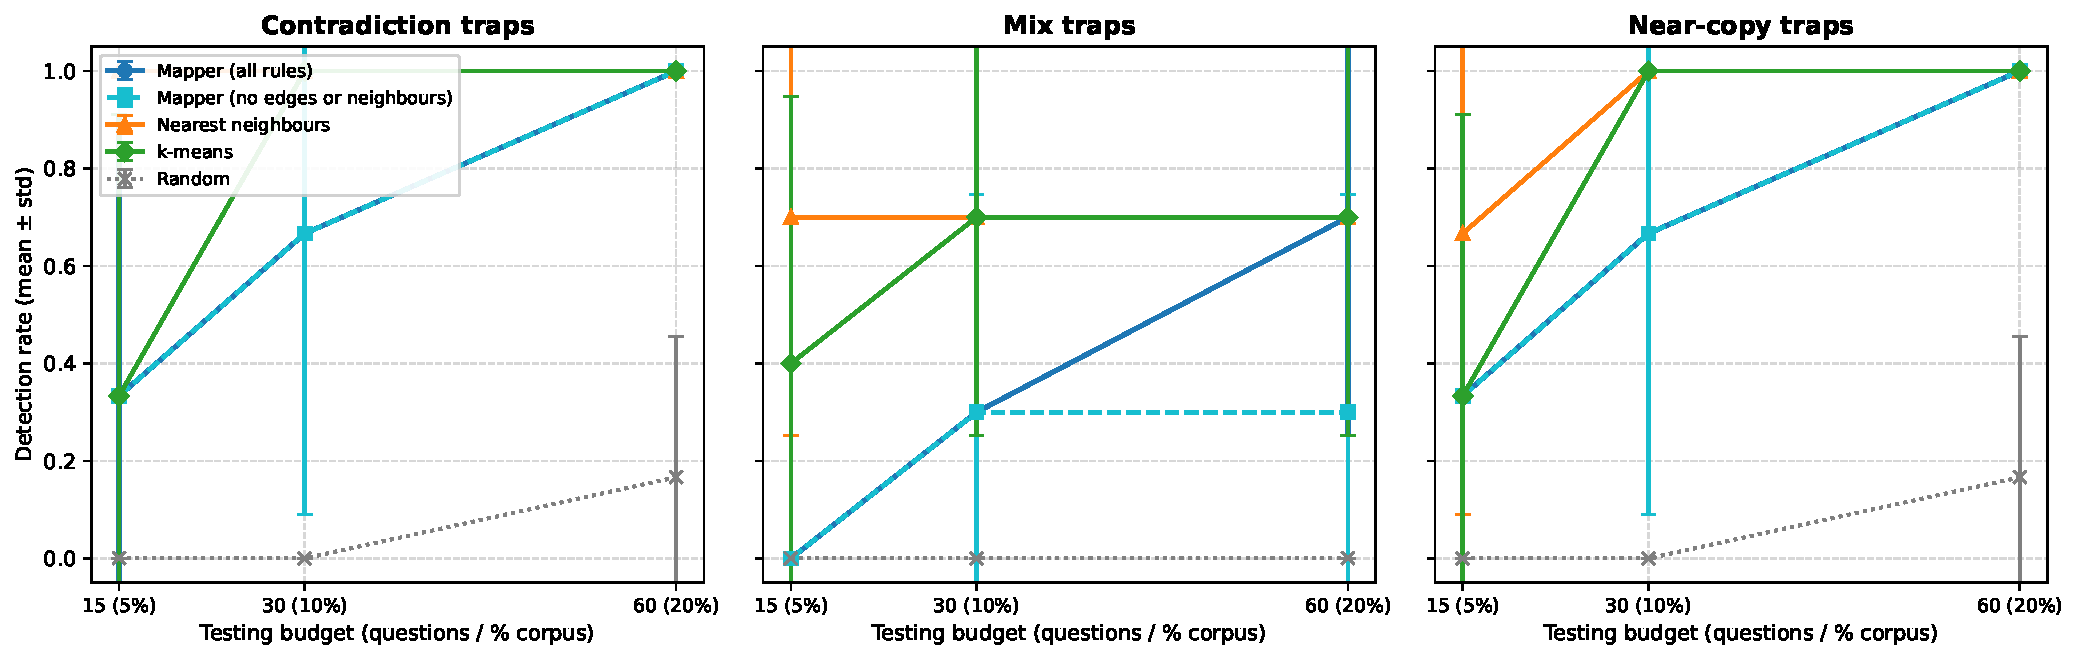
\includegraphics[width=\linewidth]{figures/main_experiment.pdf}
  \caption{Detection rate against budget for each trap type.}
  \label{fig:main-experiment}
\end{figure}

\subsection{Robustness over 100 seeds}
\label{sec:robustness}

The ten seeds above give few break events. We repeated the main experiment
with seeds 0 to 99, same corpus, selectors and budgets, on one machine. We
fixed the decision rule after seeing seeds 0 to 9 and before running seeds
10 to 99: Mapper is worse than a baseline at a
budget only if the 95\% bootstrap interval of the difference in pooled
detection rate, resampling seeds, lies below zero.
Table~\ref{tab:robustness} shows the counts and intervals. By this rule Mapper
is worse than nearest neighbours and than k-means at the three budgets. It is
above random at the three budgets.

\begin{table}[htbp]
  \centering
  \footnotesize
  \setlength{\tabcolsep}{4pt}
  \begin{tabular}{lrrr}
    \hline
    Selector & Budget 15 & Budget 30 & Budget 60 \\
    \hline
    \multicolumn{4}{l}{Broken questions found out of all break events (\%)} \\
    Mapper (all rules) & 52/232 (22.4) & 142/232 (61.2) & 195/232 (84.1) \\
    Mapper (no edges or neighbours) & 52/232 (22.4) & 140/232 (60.3) & 188/232 (81.0) \\
    Nearest neighbours & 171/232 (73.7) & 215/232 (92.7) & 216/232 (93.1) \\
    k-means & 149/232 (64.2) & 212/232 (91.4) & 216/232 (93.1) \\
    Random & 11/232 (4.7) & 22/232 (9.5) & 52/232 (22.4) \\
    \hline
    \multicolumn{4}{l}{Mapper (all rules) minus, in points [95\% interval]} \\
    Nearest neighbours & $-51.3$ & $-31.5$ & $-9.1$ \\
    & [$-61.9$, $-39.9$] & [$-39.3$, $-24.1$] & [$-13.6$, $-5.0$] \\
    k-means & $-41.8$ & $-30.2$ & $-9.1$ \\
    & [$-52.9$, $-30.6$] & [$-37.9$, $-22.7$] & [$-13.4$, $-5.2$] \\
    Random & $+17.7$ & $+51.7$ & $+61.6$ \\
    & [$+8.2$, $+27.4$] & [$+41.5$, $+61.2$] & [$+53.2$, $+69.3$] \\
    No-edges variant (post hoc) & $+0.0$ & $+0.9$ & $+3.0$ \\
    & [$+0.0$, $+0.0$] & [$+0.0$, $+2.2$] & [$+1.0$, $+5.3$] \\
    \hline
  \end{tabular}
  \caption{100 seeds, 232 break events on 10 distinct questions; the three most frequent account for 147 of them. Intervals are percentile bootstrap over seeds (10,000 draws).}
  \label{tab:robustness}
\end{table}


Only ten distinct questions ever break, and three of them account for most
break events. The intervals therefore describe these questions and this trap
generator; they do not cover the choice of other questions. The traps are
synthetic and built next to the correct chunk of each target, which may favour
nearest neighbours. The comparison without edges and neighbour expansion was
added after seeing the data: it shows no difference at budget 15, an interval
that reaches zero at budget 30, and a small gain from the graph structure at
budget 60.

A full run on another machine can differ by a few counts: restricted to seeds
0 to 9, this run finds 11 of 14 broken questions with Mapper at budget 60,
where Table~\ref{tab:main-results} reports 12 of 14.
